%package list
\documentclass{article}
\usepackage[top=3cm, bottom=3cm, outer=3cm, inner=3cm]{geometry}
\usepackage{graphicx}
\usepackage{url}
%\usepackage{cite}
\usepackage{hyperref}
\usepackage{array}
%\usepackage{multicol}
\newcolumntype{x}[1]{>{\centering\arraybackslash\hspace{0pt}}p{#1}}
\usepackage{natbib}
\usepackage{pdfpages}
\usepackage{multirow}
\usepackage{multirow}
\usepackage[normalem]{ulem}
\useunder{\uline}{\ul}{}
\usepackage{amsmath}
\usepackage{float}
\usepackage{multicol}
%%%%%%%%%%%%%%%%%%%%%%%%%%%%%%%%%%%%%%%%%%%%%%%%%%%%%%%%%%%%%%%%%%%%%%%%%%%%
%%%%%%%%%%%%%%%%%%%%%%%%%%%%%%%%%%%%%%%%%%%%%%%%%%%%%%%%%%%%%%%%%%%%%%%%%%%%
\newcommand{\csemail}{vmachacaa@ulasalle.edu.pe}
\newcommand{\csdocente}{MSc. Vicente Enrique Machaca Arceda}
\newcommand{\cscurso}{Tópicos en Computación Gráfica}
\newcommand{\csuniversidad}{Universidad San Agustín de Arequipa}
\newcommand{\csescuela}{Doctorado en Ciencias de la Computación}
\newcommand{\cspracnr}{03}
\newcommand{\cstema}{Predicción y modelado en 3D de estructuras terciarias de proteinas a partir del \textit{contact map}}
%%%%%%%%%%%%%%%%%%%%%%%%%%%%%%%%%%%%%%%%%%%%%%%%%%%%%%%%%%%%%%%%%%%%%%%%%%%%
%%%%%%%%%%%%%%%%%%%%%%%%%%%%%%%%%%%%%%%%%%%%%%%%%%%%%%%%%%%%%%%%%%%%%%%%%%%%


\usepackage[english,spanish]{babel}
\usepackage[utf8]{inputenc}
\AtBeginDocument{\selectlanguage{spanish}}
\renewcommand{\figurename}{Figura}
\renewcommand{\refname}{Referencias}
\renewcommand{\tablename}{Tabla} %esto no funciona cuando se usa babel
\AtBeginDocument{%
	\renewcommand\tablename{Tabla}
}

\usepackage{fancyhdr}
\pagestyle{fancy}
\fancyhf{}
\setlength{\headheight}{30pt}
\renewcommand{\headrulewidth}{1pt}
\renewcommand{\footrulewidth}{1pt}
\fancyhead[L]{\raisebox{-0.2\height}{
\includegraphics[width=3cm]{img/logo_unsa}}}
\fancyhead[C]{}
\fancyhead[R]{\fontsize{7}{7}\selectfont	\csuniversidad \\ \csescuela \\ \textbf{\cscurso} }
\fancyfoot[L]{MSc. Vicente Machaca}
\fancyfoot[C]{\cscurso}
\fancyfoot[R]{Página \thepage}


% para el codigo fuente
\usepackage{listings}
\usepackage{color}
\definecolor{dkgreen}{rgb}{0,0.6,0}
\definecolor{gray}{rgb}{0.5,0.5,0.5}
\definecolor{mauve}{rgb}{0.58,0,0.82}
\lstset{frame=tb,
	language=Python,
	aboveskip=3mm,
	belowskip=3mm,
	showstringspaces=false,
	columns=flexible,
	basicstyle={\small\ttfamily},
	numbers=none,
	numberstyle=\tiny\color{gray},
	keywordstyle=\color{blue},
	commentstyle=\color{dkgreen},
	stringstyle=\color{mauve},
	breaklines=true,
	breakatwhitespace=true,
	tabsize=3
}




\begin{document}
	
	\vspace*{10px}
	
	\begin{center}	
		\fontsize{17}{17} \textbf{ Avance N$^\text{o}$ \cspracnr}
	\end{center}
	%\centerline{\textbf{\underline{\Large Título: Informe de revisión del estado del arte}}}
	%\vspace*{0.5cm^
	

	\begin{table}[h]
		\begin{tabular}{|x{4cm}|x{6.3cm}|x{4cm}|}
			\hline 
			\textbf{ALUMNO} & \textbf{PROGRAMA}  & \textbf{CURSO}   \\
			\hline 
			\csdocente & \csescuela & \cscurso    \\
			\hline 
		\end{tabular}
	\end{table}	
	
	
	\begin{table}[h]
		\begin{tabular}{|x{4cm}|x{6.3cm}|x{4cm}|}
			\hline 
			\textbf{AVANCE} & \textbf{TEMA}  & \textbf{FECHA}   \\
			\hline 
			\cspracnr & \cstema & 20-02-2021 \\
			\hline 
		\end{tabular}
	\end{table}
	
	
	\section{Introducción}
	
	Las proteínas son moléculas complejas que cumplen un rol crítico en nuestro cuerpo, estas cumplen la mayoria de funciones en la células \citep{anderson1998proteome}. Además, la función de una proteína depende de su estructura \citep{rangwala2010introduction} y ultimanmente se ha descubierto que esta función tambien depende de las relación de una proteina con otras \citep{canzarprotein}. Mas aún, es importante saber, que la estructura de una proteina puede cambiar en el tiempo y su función tambien cambia en el tiempo. \\
	
	Conocer la estructura de una proteína es de suma importancia para el análisis de su función, generación de medicamentos, etc. \citep{rangwala2010introduction}. Además, lograr predecir y entender el funcionamiento de estas proteinas y la interacción de redes de proteínas es considerado el nuevo santo crial de la Binformática en estos tiempos \citep{srihari2017computational}. 
	
	
	\section{Conceptos previos}
	
	En esta sección detallaremos algunos conceptos previos del area de Bioinformática/\textit{Proteomics} para comprender el trabajo.
	
	\subsection{Estructura de las proteinas}
	
	Existen 4 tipos de estructuras de proteínas \citep{russell2002igenetics}:
	
	\begin{enumerate}
		\item \textbf{Estructura primaría:} Secuencia de aminoacidos (ver Figura \ref{fig:protein_structure} (a)).
		\item \textbf{Estructura secundaría:} Pequeños patrones, los mas comunes son las elises $\alpha$ y hojas $\beta$ (ver Figura \ref{fig:protein_structure} (b)).
		\item \textbf{Estructura terciaría:} Representa la unión de los segmentos de la estructura secundaría (ver Figura \ref{fig:protein_structure} (c)). En este caso solo estamos considerando una cadena de aminoacidos (las proteinas a veces son conformadas por varias cadenas de aminoacidos).
		\item \textbf{Estructura cuaternaría:} Union de varias estructuras terciarias (varias cadenas de aminoacidos) (ver Figura \ref{fig:protein_structure} (d)).
	\end{enumerate}
	
	
	\begin{figure}
		\centering
		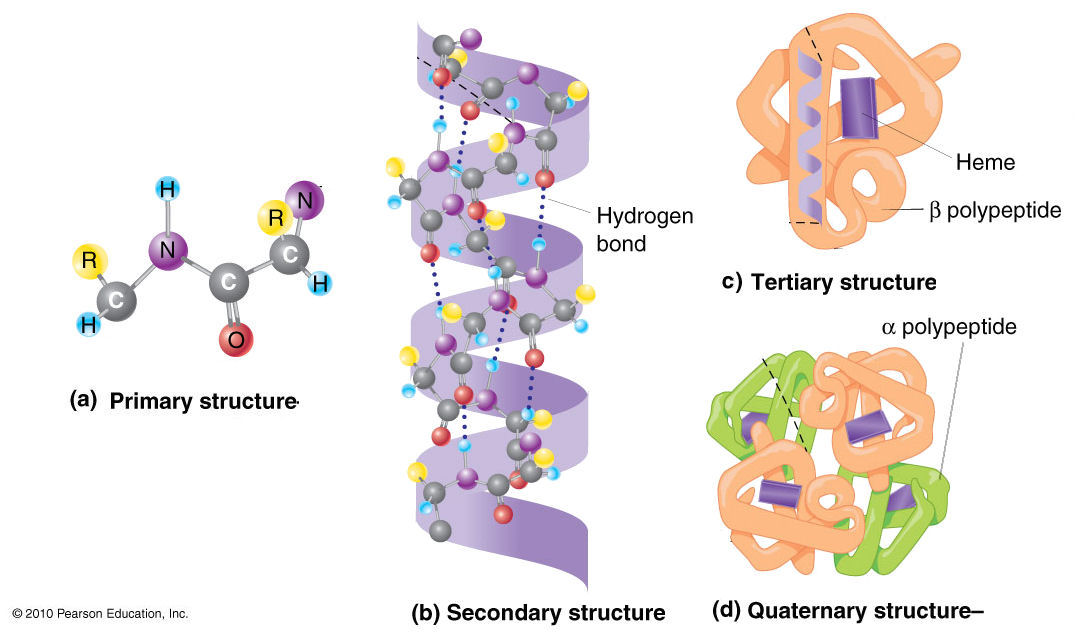
\includegraphics[width=0.6\textwidth]{img/papers/protein_structure}
		\caption{Ejemplo de las 4 estructuras de proteínas. Fuente: \citep{russell2002igenetics}}
		\label{fig:protein_structure}
	\end{figure}
	
	
	\subsection{\textit{Contact map}}
	
	Representa la distancia de cada posible aminoacido, cuando forman proteínas. El \textit{contact map}, es representado como un gráfico en 2D, y es el elegido por los modelos de machine learning en la predicción de las estructuras de proteínas. En la Figura \ref{fig:contact_map}, mostramos como es un \textit{contact map}.
	
	\begin{figure}
		\centering
		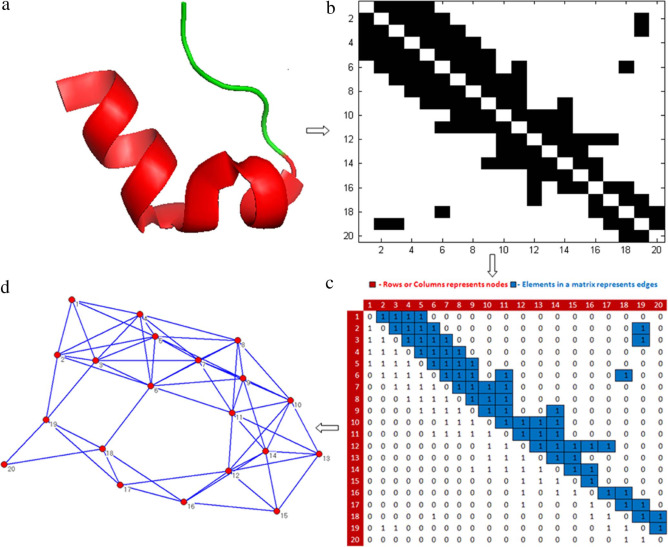
\includegraphics[width=0.4\textwidth]{img/papers/contact_map}
		\caption{Ejemplo del contact map de una proteína.}
		\label{fig:contact_map}
	\end{figure}
	
	\section{Avances}
	En esta sección, detallaremos el estado anterior del proyecto y los avances realizados estas dos ultimas semanas.
	
	\subsection{Estado anterior}
	
	Se descargo las fuentes de CONFOLD2 \cite{adhikari2018confold2} y CNS para replicar los resultados de la predicción de estructuras de proteinas a partir del \textit{contact map}. Dicha herramienta genera como salida un archivo .pdb que contiene la posición de cada atomo. Tambien se empezo el desarrollo de una herramienta que pueda visualizar los archivos .pdb, llamaremos a esta herramienta ArgosMol.
		
	\subsection{Avance y estado actual}
	
Se continuo con el desarrollo de la herramienta ArgosMol para visualizar archivos .pdb. Esta herramienta surge como una alternativa a  herramientas \textit{desktop} como: PyMol, VMD, JMol y Chimera. Además, considerando que en estos ultimos años, se ha priorizado el desarrollo de herramientas Web que hacen uso de WebGL \footnote{Librería para el desarrollo de modelos 3D. \href{https://get.webgl.org/}{Enlace.}}, 		
		Three.js \footnote{Librería de alto nivel para el desarrollo de modelos 3D, hace uso de WebGL. \href{https://threejs.org/}{Enlace.}} y 		
		3DMol.js \footnote{Librería para el modelado de átomos y moleculas, hace uso de WebGL. \href{https://threejs.org/}{Enlace.}}; 
		ArgosMol surge como como una alterntiva Web adicional, facil de usar y que sigue los principios presentados por \cite{youkharibache2017twelve}. La herramienta es presentada en la Figura \ref{fig:argos1} y esta disponible en la Web en \href{http://134.209.44.160/protein-web/3dmol/protein_interaction.php}{ArgosMol}. 
		
		
	\begin{figure}[H]
		\centering
		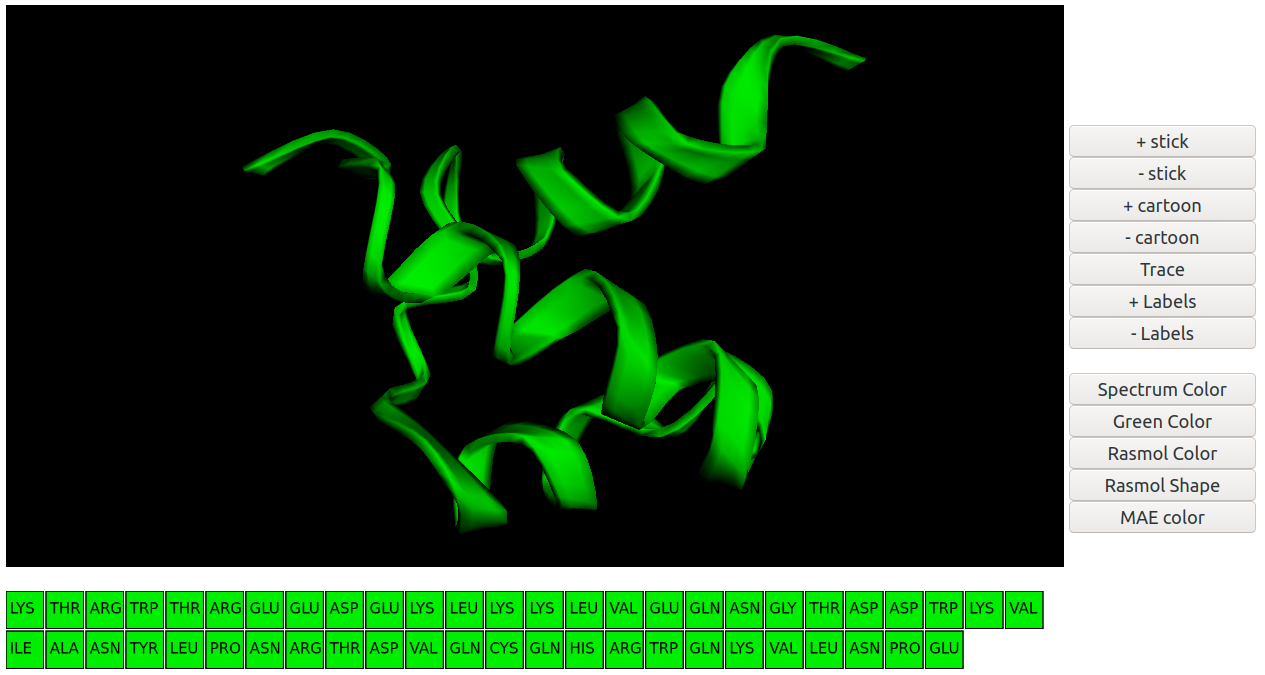
\includegraphics[width=\textwidth]{img/papers/argos1}
		\caption{ Ejemplo de visualización de proteínas con ArgosMol. }
		\label{fig:argos1}
	\end{figure}

ArgosMol es una herramienta Web para la visualización en 3D de proteínas. Está influenciada en otras herramientas Web como:

\begin{itemize}
	\item wce
\end{itemize}
	
	\clearpage
	\bibliographystyle{apalike}
	%\bibliographystyle{IEEEtranN}
	\bibliography{bibliography}
	
	
	
	
	
\end{document}